% Copyright (C)  2015  Alexander Jankowski, Philipp Hacker.
% Permission is granted to copy, distribute and/or modify this document
% under the terms of the GNU Free Documentation License, Version 1.3
% or any later version published by the Free Software Foundation;
% with no Invariant Sections, no Front-Cover Texts, and no Back-Cover Texts.
% The lincense itself can be found at <https://www.gnu.org/licenses/fdl-1.3>.

\documentclass[numbers=noenddot,a4paper]{article}
%\documentclass[numbers=noenddot,12pt,a4paper,notitlepage,twoside,BCOR15mm]{scrartcl}

\usepackage[T1]{fontenc}
\usepackage[utf8]{inputenc}

\usepackage[infoshow]{tabularx}
\usepackage[all]{xy}

\usepackage{amsmath}
\usepackage{amssymb}
\usepackage{units}
\usepackage{upgreek}
\usepackage{esint}
\usepackage{graphicx}
\usepackage{ziffer}

\usepackage{float}
\usepackage{lscape}

\usepackage[labelfont=bf]{caption}
\usepackage{wrapfig}
\usepackage{subcaption}

\usepackage[backref=page]{hyperref}

\usepackage{csquotes}
\usepackage[infoshow]{tabularx}
\usepackage{fancyhdr}

\usepackage{sectsty}
\usepackage{times}

\usepackage{paratype} %TODO Schriftart
\usepackage[greek,ngerman]{babel} %TODO Sprache einstellen

\renewcommand{\headrulewidth}{0.1pt}
\renewcommand{\footrulewidth}{0.1pt}
\newcommand{\name}{\text{Philipp Hacker}} %TODO Name des Protokollanten eintragen

\setlength{\parindent}{0pt}

\newcommand{\degree}{^\circ}
\newcommand{\diff}{\textnormal{d}}
\newcommand{\tenpo}[1]{ 10^{#1}}
\newcommand{\greek}[1]{\greektext#1\latintext}
\newcommand{\ix}[1]{_\text{#1}}
\newcommand{\imag}{\mathbf{i}}
\newcommand{\tilt}[1]{\textit{#1}}
\newcommand{\grad}[1]{\textit{grad}\left(#1\right)}
\newcommand{\divergenz}[1]{\textit{div}\left(#1\right)}
\newcommand{\euler}{\mathnormal{e}}
\newcommand{\fett}[1]{\textbf{#1}}
\newcommand{\ket}[1]{|#1\rangle}
\newcommand{\bra}[1]{\langle#1|}

\title{\fett{\underline{Protokoll: FT-IR Spektroskopie}}} %TODO Name des Versuchs eintragen
\author{Alexander Jankowski, Philipp Hacker}
\date{\today}
\pagestyle{fancy}
\fancyhead[C]{\thepage}
\fancyhead[R]{\name}
\fancyfoot[C]{\thepage}
\fancyhead[L]{Abschnitt \thesection}

\begin{document}

	\renewcommand*{\equationautorefname}{Gl.}
	\renewcommand*{\figureautorefname}{Abb.}
	\renewcommand*{\tableautorefname}{Tab.}
	\renewcommand*{\sectionautorefname}{Abschn.}
	\renewcommand*{\subsectionautorefname}{Abschn.}
	\renewcommand*{\subsubsectionautorefname}{Abschn.}
	\renewcommand*{\figurename}{Abb. }
	\renewcommand*{\tablename}{Tab.}

	\renewcommand*{\figurename}{Abbildung }
	\renewcommand*{\tablename}{Tabelle}


	\maketitle

	\begin{center}
		Betreuer: U. Martens\\ %TODO Name des Betreuers eintragen
		Versuchsdatum: 28.01.2016 \\ %TODO Datum des Versuchs eintragen
		\begin{table}[h]
			\centering
			Note: %TODO Gute Note erhalten :)
			\begin{tabularx}{1.5cm}{|X|}
				\hline \\ \\
				\hline
			\end{tabularx}
		\end{table}
	\end{center}


	\vspace*{\fill}
	\tableofcontents
	\vfill
	\clearpage

	\section{Motivation}



	\clearpage
	\section{Physikalische Grundlagen}

		

	\clearpage
	\section{Durchführung}



	\clearpage
	\section{Auswertung}

	\begin{figure}
		\includegraphics[width=\textwidth]{Gruppe2A/inter.pdf}
		\caption{Interferogramm}
		\label{img:inter}
	\end{figure}
	
	\begin{figure}
		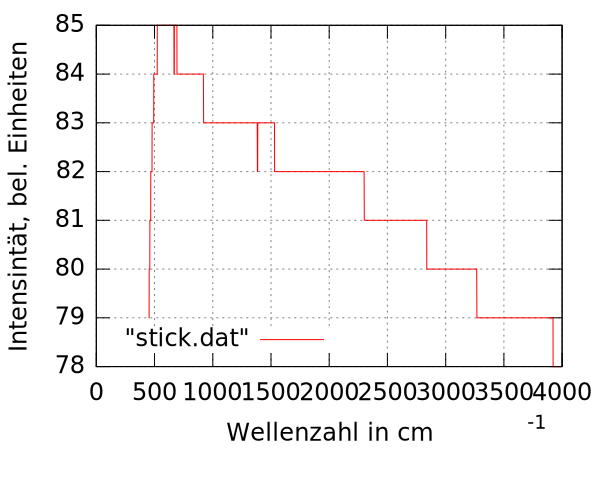
\includegraphics[width=\textwidth]{Gruppe2A/stick.pdf}
		\caption{}
		\label{img:stick}
	\end{figure}
	
	\begin{figure}
		\includegraphics[width=\textwidth]{Gruppe2A/meth.pdf}
		\caption{}
		\label{img:meth}
	\end{figure}

	\begin{figure}
		\includegraphics[width=\textwidth]{Gruppe2A/meth_diff.pdf}
		\caption{}
		\label{img:meth_diff}
	\end{figure}
	
	\clearpage
	\section{Anhang}

		\bibliography{all.bib}
		\bibliographystyle{unsrt}

\end{document}